\documentclass[12pt]{article}
\usepackage[utf8]{inputenc}
\usepackage{amsmath}
\usepackage{amsfonts}
\usepackage{amssymb}
\usepackage{graphicx}
\usepackage{hyperref}
%\graphicspath{{figures/}}
%\usepackage{color}

%%%%%%%%%%%%%%%%%%%%%%%%%%%%%%%%%%%%%%%%%%%%%%%%%%%%%%%%%%%%%%%%%%%%%
\begin{document}
\title{Metamodels and displacements  inversion \\ Notes for the R demo}
\author{Rodolphe Le Riche, Nicolas Durrande and Valérie Cayol}
%\date{15 february 2017}
\maketitle

\section{Overview}
This directory contains demo files for identifying a spherical reservoir from surface displacements. The programming language is R. 
Some data files are provided that describe the digital terrain model and the targetted surface displacements (cf. Figure~\ref{fig-piton}).
\begin{figure}
\begin{center}
\begin{minipage}{0.70\textwidth}
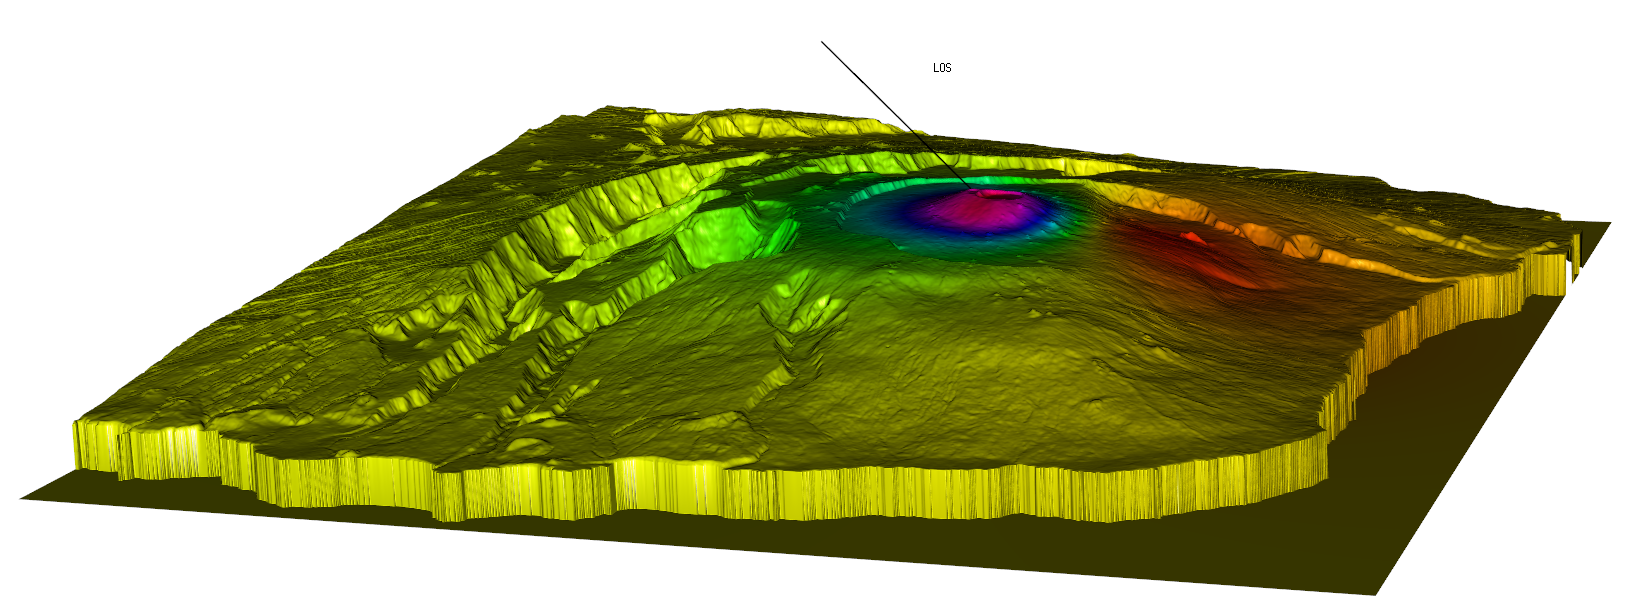
\includegraphics[width=\textwidth]{piton_ulos_2.png}
\end{minipage}
\hspace{0.05cm}
\begin{minipage}{0.44\textwidth}
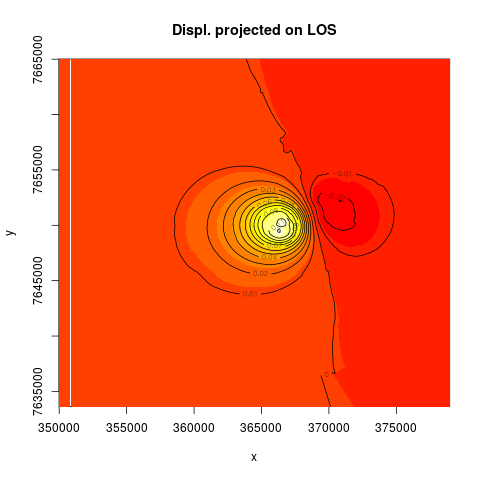
\includegraphics[width=\textwidth]{contour_ulos.png}
\end{minipage}
\end{center}
\caption{Digital terrain of the Piton de la Fournaise with displacements projected along the line of sight as colours (top) 
and (bottom) contour plot of the projected displacements (versus longitude $x$ and latitude $y$). 
These projected displacements are used in the identification.}
\label{fig-piton}
\end{figure}

The identification is performed by optimization where a distance between data (either synthetic or measured) 
and simulation results is minimized on \emph{optimization variables}. 
The spherical magma chamber is described by its position (variables $xs$, $ys$ and $zs$), its radius (variable $a$) and 
its overpressure ($p$), for a total of 5 optimization variables. The Mogi model \cite{Yamakawa1955,Mogi1958} simulates the displacements created 
by a spherical magma chamber at the surface of a digital terrain.

The optimization problem is tackled with the EGO algorithm \cite{Jones1998}. 
The generic files for the Gaussian processes and their identification can be found in the \texttt{../labSessions/} directory.
The files provided are an implementation independent from other libraries meant for both completness and simplicity.

\section{Prerequisites}
\begin{enumerate}
\item Have R available on your computer, cf. \url{https://www.r-project.org/}
\item Optionally (but really helpful) have rstudio installed, cf. \url{https://www.rstudio.com}
\item Install the \texttt{MASS} package (either from Tools / Install Package in rstudio or with the command \texttt{install.packages("MASS")}.
\item Install the \texttt{lhs} package (either from Tools / Install Package in rstudio or with the command \texttt{install.packages("lhs")}.
\item Optional: if you want to load the data that are in matlab format (\texttt{file\_name.mat}), 
install the ``R.matlab'' package (either from Tools / Install Package in rstudio or with the command \texttt{install.packages("R.matlab")}. But you can also load directly the ascii csv file (\texttt{file\_name.csv}) from R
\end{enumerate}

\section{Running the demo step by step}
\begin{enumerate}
\item Open with rstudio the file \texttt{plots\_3d\_full\_grid.R} and ``source'' it, or start R in a console in the file directory and type
\texttt{source("plots\_3d\_full\_grid.R")}. A window opens that shows the digital terrain of the volcano with a color projection of the displacements 
to be identified.
\item Open in rstudio the file \texttt{mainInversionPunctualDisplSource.R}, or open the file with any text editor and start R in a console. 
We will then proceed in steps, where each step is announced by a line of comments (\verb=#### step #####... =), and go from top to bottom. 
During each step, select sections of code with the mouse and \emph{execute} them, either (rstudio) by hitting \texttt{ctrl + return} 
or, (other text editors) by cutting and pasting in the R console. The main steps are as follows.
\item Execute \texttt{load utilities}, \texttt{input for variables identification} (where the bounds on the variables are set) and \texttt{load data}.  
\item Execute \texttt{design of experiments}: the hypercube of possible variables is filled with a Latin Hypercube Sampling. The number of points 
\texttt{nbinit}, a measure of how much randomness is devoted to the identification, is set there. 
The weighted least squares distances (WLS) to the target for each set of variables is calculated. The distances are normalized by 
$\log(1+WLS)$ follow by centering and standardization as a remedy against a large spread with outliers.
\item Execute \texttt{build a kriging model}: this means selecting a kernel for the Gaussian Process (GP) (default is \texttt{kMat52} for 
the 5/2 Mat\`ern kernel) and maximizing its log-likelihood with respect to the GP parameters (process variance and length scales).
\item Execute \texttt{test the kriging model}, which comprises creating a test set, predicting at the test variables, and measuring 
the discrepancy between the predictions and the test data (RMSE, Q2 and plots).
\item Execute \texttt{model identification}: iteratively maximize the Expected Improvement (EI) with respect to the model variables, 
update the design of experiments, and update the GP model (maximize its log-likelihood with respect to the GP parameters).
\end{enumerate}
Both the log-likelihood and the EI maximizations are performed by restarting \texttt{nbtry} times 
a BFGS algorithm with bounds on the variables from randomly chosen points. This strategy is meant to avoid getting trapped in the local 
minima that both these problems have (in particular EI).

\section{Files list}
\begin{itemize}
\item Generic files for building Gaussian Processes and optimizing with them are found in the \texttt{../labSessions/} directory. This directory
contains the complementary demo files for identifying a spherical reservoir from surface displacements.
\item \texttt{mainInversionPunctualDisplSource.R}~: main script for the demo.
\item \texttt{mogi\_3D.R}~: calculate displacements on a digital terrain model from a point-wise spherical source.
\item \texttt{plots\_3d\_full\_grid.R}~: Load a csv file (full grid), and plots its 3d data.
\item \texttt{process\_3d\_full\_grid\_from\_matlab.R}~: Load a matlab file (full grid), processes it so that it is plotted and (commented out but working) saved in csv format. Displacements are calculated with \texttt{mogi\_3D.R}.
\item \texttt{restartEGO.R}~: file specific to this demo (\texttt{mainInversionPunctualDisplSource.R}) that contains a function to restart EGO from past convergences.
\item \texttt{wls\_ulos.R}~: calculates the weighted least squares distance between the model projected displacements and the target.
\item + data files ending in \texttt{.mat} (matlab format) or \texttt{.csv} (csv format).
\end{itemize}

% BibTeX users please use one of
%\bibliographystyle{spbasic}      % basic style, author-year citations
%\bibliographystyle{spmpsci}      % mathematics and physical sciences
%\bibliographystyle{spphys}       % APS-like style for physics
\bibliographystyle{unsrt}
\bibliography{biblio_paper}   % name your BibTeX data base


\end{document}
